\section{Adoracja Krzyża}

\begin{itemize}
      \item przed ołtarzem formuje się procesja w kolejności:

            \begin{center}
                  (stopnie ołtarza) \smallskip\\
                  \cc2~~~\ii~~~~\cc1 \smallskip\\
                  \aa2~~~\aa1 \smallskip\\
                  \downarrow
            \end{center}

      \item uczestniczący w procesji skłaniają się do ołtarza, odwracają się i
            krótką drogą odchodzą do zakrystii
      \item z zakrystii \aa1 i \aa2 biorą zapalone {\color{orange} żółte} świece
            (tzw. requialne), a \ii~ zasłonięty krzyż do adoracji
      \item procesja z krzyżem przychodzi do ołtarza długą drogą w kolejności:

            \begin{center}
                  \uparrow \smallskip\\
                  \cc2~~~\cc1 \smallskip\\
                  \aa2~~~\ii~~~~\aa1\smallskip\\
            \end{center}

      \item po dojściu do ołtarza procesja staje po stronie epistoły z \aa\aa
            skierowanymi do siebie twarzami (patrz Rys. \ref{fig:crux})

            \begin{figure}[h]
                  \centering
                  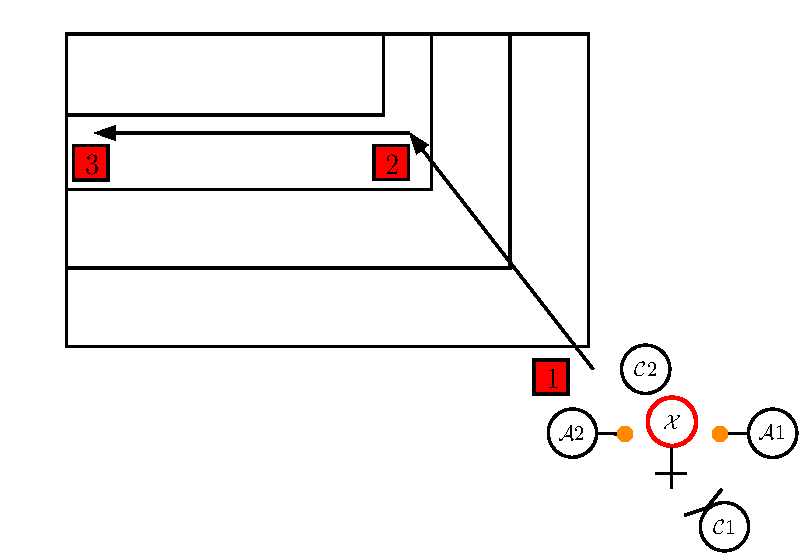
\includegraphics[scale=0.7]{Piatek/Obraz.pdf}
                  \caption{W miejscach 1,2,3 następuje odsłonięcie kolejnego
                        fragmentu krzyża; akolici są do siebie zwróceni
                        twarzami}
                  \label{fig:crux}
            \end{figure}

      \item \ii~ odsłania szczyt krzyża śpiewając \textit{Ecce lignum
                  crucis...}, na co wszyscy odpowiadają \textit{Venite,
                  adoremus}, po czym klękają (z wyjątkiem \ii)
      \item schemat powtarza się 3-krotnie: drugi raz przy ołtarzu po stronie
            epistoły (odsłaniając prawię ramię Ukrzyżowanego), a trzeci na
            środku ołtarza (odsłaniając cały krzyż)
      \item \cc2 pomaga \ii~ w odsłanianiu krzyża, za trzecim razem odbiera
            zasłonę
      \item \tt1 i \tt2 przynoszą trzy poduszki na stopnie, nakrywają je
                  {\color{violet} fioletowym} materiałem, a następnie białym
            materiałem , odbierają zasłonę od \cc2 i odnoszą ją
      \item \ii~ oddaje krzyż \cc1 i \cc2, którzy obchodzą poduszki na dół,
            przed stopniami układają krzyż na poduszkach, po czym wykonują
            wspólnie z \ii~ przyklęk i idą we trzech do sedilii
      \item \aa1 i \aa2 pozostawiają świece na najwyższym stopniu po obu
            stronach krzyża, w bezpiecznej odległości. Przyklękają po
            przeciwnych stronach krzyża i rozchodzą się na dwie strony do
            siedzeń
      \item wszyscy ściągają obuwie
      \item adoracja następuje w kolejności:

            \begin{center}
                  \ii~ \smallskip\\
                  duchowieństwo \smallskip\\
                  \cc2~~~\cc1 \smallskip\\
                  \tt2~~~\tt2 \smallskip\\
                  ministranci (dopóki nie przyjdą \aa1 i \aa2) \smallskip\\
                  \aa2~~~\aa1 \smallskip\\
                  reszta ministrantów
            \end{center}

      \item ministranci, prowadzeni przez \cc3, podchodzą do krzyża parami w
            następujący sposób (patrz także Rys. \ref{fig:adoracja}) -- każde
            klęknięcie oznacza klęknięcie na \textbf{oba kolana}:

            \begin{enumerate}[leftmargin=1cm]
                  \item pierwsze klęknięcie ma miejsce przy balaskach
                  \item drugie -- w połowie prezbiterium
                  \item trzecie -- przy stopniach ołtarza
                  \item wszystkie trzy klęknięcia wykonuje się
                        \textbf{równocześnie} z poprzedzającymi ministrantami
                  \item przy trzecim klęknięciu całuje się krzyż
                  \item po powstaniu nie przyklęka się, tylko od razu odchodzi
                        na swoje miejsce
                  \item po powrocie zakłada się obuwie i przyjmuje postawę
                        siedzącą
            \end{enumerate}

            \begin{figure}[h]
                  \centering
                  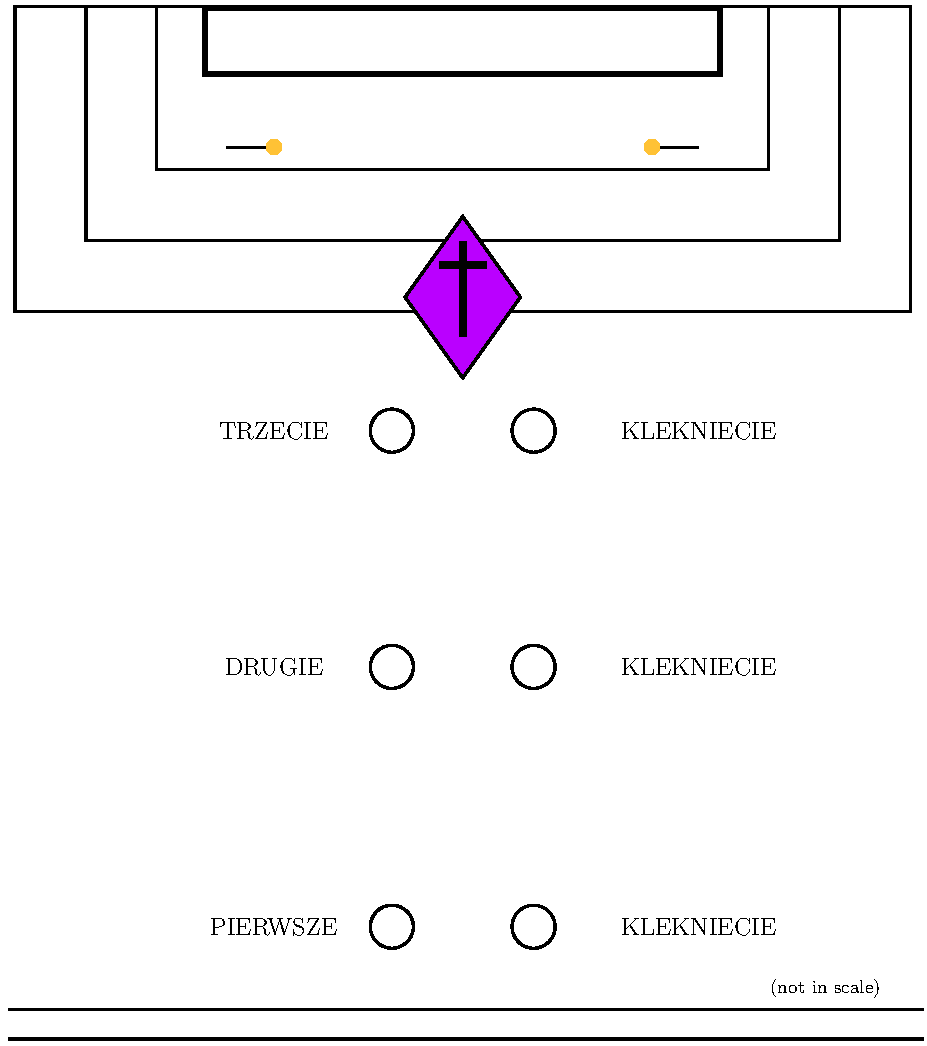
\includegraphics[scale=0.6]{Piatek/Adoracja.pdf}
                  \caption{Adoracja krzyża przez duchowieństwo i ministrantów}
                  \label{fig:adoracja}
            \end{figure}

      \item po zakończeniu adoracji przez ministrantów \cc2, trzymając już
            przygotowany ręczniczek, wraz z \tt1 zanoszą krzyż przed
            prezbiterium, w towarzystwie \aa1 i \aa2 ze świecami
      \item \aa1 i \aa2 stawiają świece na posadzce, biorą krzyż i trzymają go,
            podając wiernym do adoracji, \aa2 wyciera krzyż ręczniczkiem,
            przyniesionym przez \cc2
      \item \cc2 i \tt1 wracają do stopni ołtarza i składaja materiały fioletowy
            i biały, zbierają poduszki,
      \item następuje adoracja krzyża przez wiernych
      \item dwaj wyznaczeni ministranci przynoszą koszyczki na tacę i stają z
            nimi po obu stronach krzyża
      \item w czasie adoracji \ii~ siedząc na sedilli odczytuje
            \textit{Improperia} z księgi OHS trzymanej przez \bb;
      \item w tym czasie \cc2 i \tt1 zanoszą na ołtarz {\color{violet}
            fioletową} bursę z korporałem, który rozkładają, oraz vasculum z
            ręczniczkiem, mszał przesuwają nieco na stronę ewangelii
      \item \tt1 i \tt2 wychodzą przygotować kadzidło
      \item \zz~ przynosi przed ołtarz schodki do ustawienia krzyża w podstawie
      \item po zakończonej adoracji \ii~ odbiera krzyż, po czym wraz z \cc1 i
            wyznaczonym wcześniej wysokim ministrantem \mm~ zanoszą krzyż na
            ołtarz i umieszczają w podstawie, wówczas wszyscy \textbf{wstają}
      \item \aa1 i \aa2 towarzyszą w odnoszeniu krzyża, po czym zostawiają
            świece na ołtarzu (jak najbliżej tabernakulum), wszyscy schodzą
            przed stopnie, przyklękają i wracają na swoje miejsca

            \begin{center}
                  (stopnie ołtarza) \smallskip\\
                  \mm~~\ii~~\cc1 \smallskip\\
                  \aa1~~~~~\aa2
            \end{center}

      \item \cc2 zabiera schodki
\end{itemize}
